\documentclass[12pt,a4paper]{article}
\usepackage[utf8]{inputenc}
\usepackage{fontspec}
\usepackage{geometry}
\usepackage{graphicx}
\usepackage{fancyhdr}
\usepackage{titlesec}
\usepackage{amsmath}
\usepackage{amsfonts}
\usepackage{amssymb}
\usepackage{booktabs}
\usepackage{longtable}
\usepackage{array}
\usepackage{multirow}
\usepackage{multicol}
\usepackage{xcolor}
\usepackage{colortbl}
\usepackage{tikz}
\usepackage{pgfplots}
\usepackage{pgf-pie}
\usepackage{hyperref}
\usepackage{enumitem}
\usepackage{float}
\usepackage{caption}
\usepackage{subcaption}
\usepackage{listings}
\usepackage{textcomp}
\usepackage{gensymb}
\usepackage{siunitx}
\usepackage{acronym}
\usepackage{glossaries}
\usepackage{pdfpages}
\usepackage{rotating}
\usepackage{pdflscape}
\usepackage{afterpage}
\usepackage{placeins}

% Set Times New Roman as main font
\setmainfont{Times New Roman}
\setsansfont{Arial}
\setmonofont{Courier New}

% Page geometry
\geometry{
    left=2.5cm,
    right=2.5cm,
    top=2.5cm,
    bottom=2.5cm,
    headheight=1.8cm,
    headsep=0.5cm,
    footskip=1cm
}

% Colors
\definecolor{spitblue}{RGB}{0,51,102}
\definecolor{spitgold}{RGB}{255,204,0}
\definecolor{darkblue}{RGB}{0,31,63}
\definecolor{lightblue}{RGB}{173,216,230}
\definecolor{gray}{RGB}{128,128,128}
definecolor{lightgreen}{RGB}{144,238,144}
\definecolor{lightyellow}{RGB}{255,255,224}
\definecolor{lightcoral}{RGB}{240,128,128}
\definecolor{plum}{RGB}{221,160,221}
\definecolor{wheat}{RGB}{245,222,179}

% Hyperref settings
\hypersetup{
    colorlinks=true,
    linkcolor=spitblue,
    filecolor=spitblue,
    urlcolor=spitblue,
    citecolor=spitblue,
    pdftitle={AEGIS: Advanced Enterprise Grid & Industrial Security Platform},
    pdfauthor={Bharatiya Vidya Bhavan's Sardar Patel Institute of Technology},
    pdfsubject={Government Research Proposal},
    pdfkeywords={Cybersecurity, OT Security, Industrial Control Systems, Smart Grid}
}

% Header and footer
\pagestyle{fancy}
\fancyhf{}
\fancyhead[L]{
\includegraphics[width=2.5cm]{spit_logo.png}}
\fancyhead[C]{\textbf{\footnotesize AEGIS Research Proposal - Government Format}}
\fancyhead[R]{\footnotesize Page \thepage}
\fancyfoot[C]{\footnotesize Bharatiya Vidya Bhavan's Sardar Patel Institute of Technology}
\renewcommand{\headrulewidth}{0.4pt}
\renewcommand{\footrulewidth}{0.4pt}

% Title formatting
\titleformat{\section}
{\color{spitblue}\normalfont\Large\bfseries}
{\color{spitblue}\thesection}{1em}{}

\titleformat{\subsection}
{\color{darkblue}\normalfont\large\bfseries}
{\color{darkblue}\thesubsection}{1em}{}

\titleformat{\subsubsection}
{\color{darkblue}\normalfont\normalsize\bfseries}
{\color{darkblue}\thesubsubsection}{1em}{}

% Custom commands
\newcommand{\rupees}{Rs.\,}
\newcommand{\crores}{\text{ Crores}}
\newcommand{\lakhs}{\text{ Lakhs}}

% Table settings
\renewcommand{\arraystretch}{1.2}

% Glossary
\makeglossaries
\newacronym{ot}{OT}{Operational Technology}
\newacronym{it}{IT}{Information Technology}
\newacronym{ics}{ICS}{Industrial Control Systems}
\newacronym{scada}{SCADA}{Supervisory Control and Data Acquisition}
\newacronym{ai}{AI}{Artificial Intelligence}
\newacronym{ml}{ML}{Machine Learning}

\begin{document}

% Government Format Title Page
\begin{titlepage}
    \centering
    
    % Logo
    \vspace*{-1cm}
    
\includegraphics[width=4cm]{spit_logo.png}
    
    \vspace{0.5cm}
    
    {\Large\textbf{BHARATIYA VIDYA BHAVAN'S}\\[0.2cm]}
    {\Large\textbf{SARDAR PATEL INSTITUTE OF TECHNOLOGY}\\[0.3cm]}
    {\normalsize Munshi Nagar, Andheri (West), Mumbai - 400058, Maharashtra, India\\[0.8cm]}
    
    \vspace{0.5cm}
    
    % Government Format Header
    {\color{spitblue}\LARGE\textbf{PROFORMA FOR SUBMITTING R\&D PROJECT PROPOSAL}}\\[0.3cm]
    {\color{spitblue}\LARGE\textbf{FOR SEEKING FINANCIAL SUPPORT}}\\[1cm]
    
    % Title
    {\color{darkblue}\Huge\textbf{AEGIS}}\\[0.4cm]
    {\color{darkblue}\Large\textbf{Advanced Enterprise Grid \& Industrial Security Platform}}\\[0.3cm]
    {\large A Next-Generation Distributed OT/IT Cybersecurity Ecosystem}\\[1cm]
    
    % Project details box
    \begin{center}
    \fbox{\begin{minipage}{0.85\textwidth}
        \centering
        \textbf{Project Title:} AEGIS: Advanced Enterprise Grid \& Industrial Security Platform\\[0.2cm]
        \textbf{Total Budget:} \rupees 4,70,00,000 (4.7 Crores)\\[0.2cm]
        \textbf{Duration:} 36 Months (3 Years)\\[0.2cm]
        \textbf{Proposal Date:} \today\\[0.2cm]
        \textbf{Classification:} Strategic National Infrastructure Protection Initiative\\[0.2cm]
        \textbf{Nature:} R,D \& E leading to production capability + Application oriented R,D\&D
    \end{minipage}}
    \end{center}
    
    \vfill
    
    % Bottom information
    {\large\textbf{Submitted to:} Government of India\\[0.2cm]}
    {\normalsize Department of Electronics and Information Technology (DeitY)\\[0.2cm]}
    {\normalsize Under the National Cybersecurity Research Initiative\\[0.2cm]}
    {\normalsize for Critical Infrastructure Protection}
    
    \vspace{1cm}
    
    {\footnotesize Document Version: 4.0 Government Format | Classification: Confidential - Government Use Only}
    
\end{titlepage}

\newpage

% PART 1: SUMMARY SHEET (Government Format)
\section*{PROFORMA FOR SUBMITTING R\&D PROJECT PROPOSAL}
\section*{FOR SEEKING FINANCIAL SUPPORT}
\section*{SUMMARY SHEET}

\begin{longtable}{|p{0.5cm}p{3cm}|p{11cm}|}
\hline
\rowcolor{lightblue}
\multicolumn{2}{|c|}{\textbf{Field}} & \textbf{Details} \\
\hline
\endhead

\multicolumn{2}{|l|}{\textbf{1.}} & \textbf{Title of Project} \\
\multicolumn{2}{|l|}{} & AEGIS: Advanced Enterprise Grid \& Industrial Security Platform - A Next-Generation Distributed OT/IT Cybersecurity Ecosystem \\
\hline

\multicolumn{2}{|l|}{\textbf{2.}} & \textbf{Organisation} \\
\multicolumn{2}{|l|}{a)} & \textbf{Name:} Bharatiya Vidya Bhavan's Sardar Patel Institute of Technology (SPIT) \\
\multicolumn{2}{|l|}{b)} & \textbf{Address:} Munshi Nagar, Andheri (West), Mumbai - 400058, Maharashtra, India \\
\multicolumn{2}{|l|}{c)} & \textbf{Legal status:} Autonomous Institute under Bharatiya Vidya Bhavan (Registered Trust under Bombay Public Trust Act, 1950). Educational Institution recognized by UGC and AICTE. \\
\hline

\multicolumn{2}{|l|}{\textbf{3.}} & \textbf{Chief Investigator} \\
\multicolumn{2}{|l|}{a)} & \textbf{Name:} Dr. [To be appointed - Senior Professor with 15+ years experience in Cybersecurity] \\
\multicolumn{2}{|l|}{b)} & \textbf{Designation:} Principal Investigator \& Project Director \\
\multicolumn{2}{|l|}{c)} & \textbf{Department:} Electronics \& Telecommunications Engineering / Computer Engineering \\
\multicolumn{2}{|l|}{d)} & \textbf{Address:} SPIT, Munshi Nagar, Andheri (West), Mumbai - 400058, Maharashtra \\
\hline

\multicolumn{2}{|l|}{\textbf{4.}} & \textbf{Nature of Project (Check one)} \\
\multicolumn{2}{|l|}{} & $\checkmark$ \textbf{a) Research, Development \& Engineering (R,D \& E) leading to production capability} \\
\multicolumn{2}{|l|}{} & $\checkmark$ \textbf{b) Application oriented Research, Design and Development (R,D\&D) having production potential} \\
\multicolumn{2}{|l|}{} & c) Basic R\&D \\
\hline

\multicolumn{2}{|l|}{\textbf{5.}} & \textbf{Objective of the Project} \\
\multicolumn{2}{|l|}{} & 
\begin{itemize}[leftmargin=1em, itemsep=0pt]
    \item Develop indigenous distributed OT/IT cybersecurity platform for critical infrastructure
    \item Implement quantum-resistant encryption for industrial protocols (50+ protocols supported)
    \item Create AI-powered threat detection system with 99.5\% accuracy and <0.1\% false positive rate
    \item Build blockchain-based forensic audit system for tamper-proof logging
    \item Design hardware data diode for air-gapped security (10Gbps throughput)
    \item Establish comprehensive protocol intelligence platform supporting DNP3, IEC 61850, Modbus, OPC UA, MQTT, and 45+ other industrial protocols
    \item Develop real-time 3D visualization and command center with AR/VR support
    \item Create automated incident response framework with SOAR integration
\end{itemize} \\
\hline

\end{longtable}

\newpage

\begin{longtable}{|p{0.5cm}p{3cm}|p{11cm}|}
\hline
\rowcolor{lightblue}
\multicolumn{2}{|c|}{\textbf{Field}} & \textbf{Details} \\
\hline
\endhead

\multicolumn{2}{|l|}{\textbf{6.}} & \textbf{Brief outline of the project with specific technology fall-outs} \\
\multicolumn{2}{|l|}{} & 
\textbf{Project Scope:} AEGIS is a comprehensive OT/IT cybersecurity ecosystem comprising 8 integrated modules:
\begin{enumerate}[leftmargin=1em, itemsep=0pt]
    \item \textbf{AssetGuard} - Intelligent Asset Discovery Engine with 99.5\% device identification accuracy
    \item \textbf{ProtoSense} - Universal Protocol Intelligence Platform supporting 50+ industrial protocols
    \item \textbf{ThreatHunter} - AI-Powered Threat Detection System with advanced ML algorithms
    \item \textbf{ChainAudit} - Blockchain-Powered Forensic System for immutable audit trails
    \item \textbf{DiodeGuard} - Hardware-Accelerated Data Diode (10Gbps, FIPS 140-2 Level 3)
    \item \textbf{VizDash} - Advanced 3D Visualization \& Command Center with AR/VR support
    \item \textbf{LogMiner} - Intelligent Log Processing System with real-time analytics
    \item \textbf{AlertStream} - Automated Incident Response Orchestrator with SOAR integration
\end{enumerate}

\textbf{Specific Technology Fall-outs:}
\begin{itemize}[leftmargin=1em, itemsep=0pt]
    \item Post-quantum cryptographic algorithms (CRYSTALS-Kyber, SPHINCS+)
    \item Industrial AI/ML models for behavioral anomaly detection
    \item Custom FPGA-based protocol parsers with hardware acceleration
    \item Permissioned blockchain architecture for audit trail management
    \item Zero-trust security architecture specifically designed for OT environments
    \item Custom hardware data diode with optical isolation technology
    \item Real-time 3D network visualization engine with immersive interfaces
    \item Automated playbook execution engine for incident response
    \item Indigenous hardware security modules (HSM) design
    \item Edge computing framework for distributed threat detection
\end{itemize} \\
\hline

\multicolumn{2}{|l|}{\textbf{7.}} & \textbf{Expected outcome in physical terms} \\
\multicolumn{2}{|l|}{a)} & \textbf{Specifications of subsystem/system:}
\begin{itemize}[leftmargin=1em, itemsep=0pt]
    \item System Throughput: 1M+ events/second with <100ms response latency
    \item Protocol Support: 50+ industrial protocols including DNP3, IEC 61850, Modbus, OPC UA
    \item Scalability: Support for 10,000+ devices per deployment instance
    \item Availability: 99.99\% uptime with redundant architecture
    \item Detection Accuracy: 99.5\% threat detection with <0.1\% false positive rate
    \item Data Retention: 7 years with compressed storage optimization
    \item Hardware: Custom data diode (10Gbps), HSM integration, FPGA acceleration
    \item Compliance: FIPS 140-2 Level 3, ISO 27001, IEC 62443 SL-3 capable
\end{itemize} \\

\multicolumn{2}{|l|}{b)} & \textbf{Nature of documents for technology transfer:}
\begin{itemize}[leftmargin=1em, itemsep=0pt]
    \item 15+ patent applications in cybersecurity, protocol analysis, and hardware security
    \item Complete source code repository with comprehensive documentation (1000+ pages)
    \item Technical implementation guides and API documentation
    \item Hardware design specifications and FPGA implementations
    \item Training manuals and certification programs
    \item Compliance and standards mapping documentation
    \item Deployment and installation guides for various environments
    \item Performance benchmarking and testing methodologies
\end{itemize} \\

\multicolumn{2}{|l|}{c)} & \textbf{Manpower trained:} \\
\multicolumn{2}{|l|}{i)} & \textbf{Level of training:} Graduate/Post-graduate engineers, Industry professionals, Government officials \\
\multicolumn{2}{|l|}{ii)} & \textbf{Numbers:} 
\begin{itemize}[leftmargin=1em, itemsep=0pt]
    \item \textbf{Internal (R\&D):} 60+ researchers, engineers, and support staff
    \item \textbf{Industry:} 200+ professionals through certification programs
    \item \textbf{Outside R\&D:} 300+ government officials, security analysts, and operators
    \item \textbf{Total:} 560+ trained personnel across different categories
\end{itemize} \\
\hline

\end{longtable}

\newpage

\begin{longtable}{|p{0.5cm}p{3cm}|p{11cm}|}
\hline
\rowcolor{lightblue}
\multicolumn{2}{|c|}{\textbf{Field}} & \textbf{Details} \\
\hline
\endhead

\multicolumn{2}{|l|}{\textbf{8.}} & \textbf{Agency with which link up is established/proposed} \\
\multicolumn{2}{|l|}{} & 
\textbf{Government Agencies:}
\begin{itemize}[leftmargin=1em, itemsep=0pt]
    \item Power Grid Corporation of India (POWERGRID) - Smart grid security testing
    \item Indian Computer Emergency Response Team (CERT-In) - Threat intelligence sharing
    \item National Critical Information Infrastructure Protection Centre (NCIIPC) - Standards compliance
    \item Defence Research and Development Organisation (DRDO) - Defense applications
    \item Centre for Development of Advanced Computing (C-DAC) - HPC integration
    \item Bureau of Indian Standards (BIS) - Standards development
\end{itemize}

\textbf{Industry Partners:}
\begin{itemize}[leftmargin=1em, itemsep=0pt]
    \item Tata Consultancy Services (TCS) - System integration and deployment
    \item Larsen \& Toubro (L\&T) - Hardware manufacturing and testing
    \item Bharti Airtel - Network infrastructure and 5G integration
    \item Oil \& Natural Gas Corporation (ONGC) - Pilot deployment in energy sector
    \item Nuclear Power Corporation of India (NPCIL) - Critical infrastructure testing
\end{itemize}

\textbf{Academic Collaborations:}
\begin{itemize}[leftmargin=1em, itemsep=0pt]
    \item Indian Institute of Technology (IIT) Delhi - AI/ML research collaboration
    \item Indian Institute of Science (IISc) Bangalore - Quantum computing research
    \item International partnerships with Carnegie Mellon University (USA), Technical University of Denmark
\end{itemize} \\
\hline

\multicolumn{2}{|l|}{\textbf{9.}} & \textbf{Duration of Project:} 36 Months (3 Years) \\
\hline

\end{longtable}

% Year-wise breakdown table
\section*{10. Year-wise break-up of physical achievements with specific intermediate milestones}

\begin{longtable}{|p{2cm}|p{4cm}|p{8.5cm}|}
\hline
\rowcolor{lightblue}
\textbf{Year} & \textbf{Phase} & \textbf{Physical Achievements \& Milestones} \\
\hline
\endhead

\multirow{8}{*}{\textbf{Year 1}} & \textbf{Foundation Phase} & 
\textbf{Q1 (Oct-Dec 2024):}
\begin{itemize}[leftmargin=1em, itemsep=0pt]
    \item Team recruitment (60+ experts across domains)
    \item Infrastructure setup (High-end GPU servers, network equipment)
    \item Test lab establishment with industrial equipment
    \item Initial protocol analysis framework for 10 protocols
\end{itemize}

\textbf{Milestone M1:} Team and infrastructure ready \\
\cline{2-3}

& \textbf{Core Development} & 
\textbf{Q2 (Jan-Mar 2025):}
\begin{itemize}[leftmargin=1em, itemsep=0pt]
    \item AssetGuard alpha version with device discovery
    \item ProtoSense parser development for DNP3, Modbus, IEC 61850
    \item Initial security framework design and implementation
    \item Hardware data diode prototype development
\end{itemize}

\textbf{Milestone M2:} Core modules alpha release \\
\cline{2-3}

& \textbf{Protocol Integration} & 
\textbf{Q3 (Apr-Jun 2025):}
\begin{itemize}[leftmargin=1em, itemsep=0pt]
    \item ThreatHunter ML model development and training
    \item ChainAudit blockchain integration
    \item Protocol support expansion to 25+ protocols
    \item Initial performance testing and optimization
\end{itemize}

\textbf{Milestone M3:} Protocol intelligence platform operational \\
\cline{2-3}

& \textbf{Testing \& Validation} & 
\textbf{Q4 (Jul-Sep 2025):}
\begin{itemize}[leftmargin=1em, itemsep=0pt]
    \item System integration and testing
    \item Security audit and penetration testing
    \item Performance benchmarking (target: 100K events/sec)
    \item Documentation and user manual development
\end{itemize}

\textbf{Milestone M4:} Year 1 system validation complete \\
\hline

\end{longtable}

\newpage

\begin{longtable}{|p{2cm}|p{4cm}|p{8.5cm}|}
\hline
\rowcolor{lightblue}
\textbf{Year} & \textbf{Phase} & \textbf{Physical Achievements \& Milestones} \\
\hline
\endhead

\multirow{8}{*}{\textbf{Year 2}} & \textbf{Advanced Features} & 
\textbf{Q1 (Oct-Dec 2025):}
\begin{itemize}[leftmargin=1em, itemsep=0pt]
    \item Complete protocol support (50+ protocols)
    \item AI/ML model optimization (target: 95\% accuracy)
    \item VizDash 3D visualization system development
    \item Quantum-resistant encryption implementation
\end{itemize}

\textbf{Milestone M5:} Advanced features integration \\
\cline{2-3}

& \textbf{ML/AI Integration} & 
\textbf{Q2 (Jan-Mar 2026):}
\begin{itemize}[leftmargin=1em, itemsep=0pt]
    \item LogMiner analytics engine with real-time processing
    \item Advanced threat detection with behavioral analysis
    \item Zero-trust architecture implementation for OT networks
    \item Edge computing deployment framework
\end{itemize}

\textbf{Milestone M6:} AI/ML platform fully operational \\
\cline{2-3}

& \textbf{Security Enhancement} & 
\textbf{Q3 (Apr-Jun 2026):}
\begin{itemize}[leftmargin=1em, itemsep=0pt]
    \item AlertStream automation engine with SOAR integration
    \item Hardware data diode production version (10Gbps)
    \item Blockchain forensics system with smart contracts
    \item Compliance certification preparation (ISO 27001, IEC 62443)
\end{itemize}

\textbf{Milestone M7:} Security platform hardening complete \\
\cline{2-3}

& \textbf{System Integration} & 
\textbf{Q4 (Jul-Sep 2026):}
\begin{itemize}[leftmargin=1em, itemsep=0pt]
    \item Full system integration testing
    \item Performance optimization (target: 1M events/sec)
    \item Beta testing with selected industry partners
    \item Regulatory compliance validation
\end{itemize}

\textbf{Milestone M8:} Integrated platform ready for deployment \\
\hline

\multirow{8}{*}{\textbf{Year 3}} & \textbf{Pilot Deployment} & 
\textbf{Q1 (Oct-Dec 2026):}
\begin{itemize}[leftmargin=1em, itemsep=0pt]
    \item Pilot deployment at 3 critical infrastructure sites
    \item Real-world testing with power grid, oil \& gas facilities
    \item Performance validation and optimization
    \item User training and certification program launch
\end{itemize}

\textbf{Milestone M9:} Successful pilot deployments \\
\cline{2-3}

& \textbf{Performance Tuning} & 
\textbf{Q2 (Jan-Mar 2027):}
\begin{itemize}[leftmargin=1em, itemsep=0pt]
    \item Scaling to additional pilot sites (total 5 sites)
    \item Performance tuning based on real-world feedback
    \item Advanced features refinement and optimization
    \item Industry partnerships for commercialization
\end{itemize}

\textbf{Milestone M10:} Production-ready platform \\
\cline{2-3}

& \textbf{Documentation} & 
\textbf{Q3 (Apr-Jun 2027):}
\begin{itemize}[leftmargin=1em, itemsep=0pt]
    \item Comprehensive technical documentation (1000+ pages)
    \item Patent filing for 15+ innovations
    \item Training material development and certification programs
    \item Standards contribution and white paper publications
\end{itemize}

\textbf{Milestone M11:} Complete documentation and IP protection \\
\cline{2-3}

& \textbf{Project Completion} & 
\textbf{Q4 (Jul-Sep 2027):}
\begin{itemize}[leftmargin=1em, itemsep=0pt]
    \item Technology transfer to industry partners
    \item Final project evaluation and assessment
    \item Sustainability and commercialization plan execution
    \item Project handover and closure activities
\end{itemize}

\textbf{Milestone M12:} Project successfully completed \\
\hline

\end{longtable}

\newpage

\begin{longtable}{|p{0.5cm}p{3cm}|p{11cm}|}
\hline
\rowcolor{lightblue}
\multicolumn{2}{|c|}{\textbf{Field}} & \textbf{Details} \\
\hline
\endhead

\multicolumn{2}{|l|}{\textbf{11.}} & \textbf{Likely End User(s)} \\
\multicolumn{2}{|l|}{} & 
\textbf{Primary End Users (Critical Infrastructure):}
\begin{itemize}[leftmargin=1em, itemsep=0pt]
    \item \textbf{Power Sector:} Power Grid Corporation of India, State Electricity Boards, NTPC, NHPC
    \item \textbf{Oil \& Gas:} ONGC, IOC, GAIL, Reliance Industries, petrochemical complexes
    \item \textbf{Nuclear:} Nuclear Power Corporation of India (NPCIL), BARC, nuclear facilities
    \item \textbf{Transportation:} Indian Railways, Delhi Metro, Mumbai Metro, airport authorities
    \item \textbf{Smart Cities:} 100+ Smart City Mission projects, municipal corporations
    \item \textbf{Defense:} Indian Armed Forces, defense PSUs, strategic installations
    \item \textbf{Water:} Water treatment plants, irrigation systems, municipal water supplies
    \item \textbf{Manufacturing:} Steel plants (SAIL, Tata Steel), automotive, pharma industries
\end{itemize}

\textbf{Secondary Markets:}
\begin{itemize}[leftmargin=1em, itemsep=0pt]
    \item International clients in BRICS nations and friendly countries
    \item Private industrial enterprises and commercial facilities
    \item Cybersecurity service providers and system integrators
    \item Academic institutions and research organizations
\end{itemize} \\
\hline

\multicolumn{2}{|l|}{\textbf{12.}} & \textbf{Name of other organisations jointly participating in the project} \\
\multicolumn{2}{|l|}{} & 
\textbf{Domestic Collaborative Organizations:}
\begin{itemize}[leftmargin=1em, itemsep=0pt]
    \item \textbf{Indian Institute of Technology (IIT) Delhi} - AI/ML research, algorithm development
    \item \textbf{Indian Institute of Science (IISc) Bangalore} - Quantum computing, cryptographic research
    \item \textbf{Centre for Development of Advanced Computing (C-DAC)} - High-performance computing integration
    \item \textbf{Tata Consultancy Services (TCS)} - System integration, software development
    \item \textbf{Larsen \& Toubro (L\&T)} - Hardware manufacturing, industrial deployment
    \item \textbf{Bharti Airtel} - Network infrastructure, 5G integration testing
\end{itemize}

\textbf{International Collaborating Organizations:}
\begin{itemize}[leftmargin=1em, itemsep=0pt]
    \item \textbf{Carnegie Mellon University, USA} - Industrial Control Systems security research
    \item \textbf{Technical University of Denmark} - Smart grid cybersecurity collaboration
    \item \textbf{Fraunhofer Institute, Germany} - Industrial cybersecurity standards and testing
    \item \textbf{National Institute of Standards and Technology (NIST), USA} - Standards development
\end{itemize} \\
\hline

\end{longtable}

\newpage

% Budget Section - Government Format
\section*{13. Total Budget outlay (Rs. in lakhs)}

\begin{table}[H]
\centering
\caption{Budget Breakdown - 3 Year Project Timeline}
\renewcommand{\arraystretch}{1.4}
\begin{tabular}{|p{3.5cm}|c|c|c|c|}
\hline
\rowcolor{lightblue}
\textbf{Head} & \textbf{1st Year} & \textbf{2nd Year} & \textbf{3rd Year} & \textbf{Total} \\
& \textbf{(Rs. Lakhs)} & \textbf{(Rs. Lakhs)} & \textbf{(Rs. Lakhs)} & \textbf{(Rs. Lakhs)} \\
\hline

\textbf{Capital Equipment} & 80.0 & 60.0 & 40.0 & \textbf{180.0} \\
\hline

\textbf{Consumable stores} & 15.0 & 12.0 & 8.0 & \textbf{35.0} \\
\hline

\textbf{Manpower} & 80.0 & 70.0 & 60.0 & \textbf{210.0} \\
\hline

\textbf{Travel \& Training} & 8.0 & 7.0 & 5.0 & \textbf{20.0} \\
\hline

\textbf{Contingencies including TA/DA for Project review meetings} & 5.0 & 4.0 & 3.0 & \textbf{12.0} \\
\hline

\textbf{Overheads, if any} & 12.0 & 10.0 & 8.0 & \textbf{30.0} \\
\hline

\rowcolor{yellow}
\textbf{Grand Total} & \textbf{200.0} & \textbf{163.0} & \textbf{124.0} & \textbf{487.0} \\
\hline

\end{tabular}
\end{table}

\section*{14. Grand Total: Rs. 487.0 Lakhs (4.87 Crores)}

\begin{table}[H]
\centering
\renewcommand{\arraystretch}{1.4}
\begin{tabular}{|p{8cm}|c|}
\hline
\rowcolor{lightblue}
\textbf{Funding Source} & \textbf{Amount (Rs. Lakhs)} \\
\hline

\textbf{a) Contribution of Project Implementing \& other Organisation in Total Budget Outlay} & 48.7 \\
\textbf{(10\% matching contribution from SPIT and industry partners)} & \\
\hline

\textbf{b) DeitY Contribution} & \textbf{438.3} \\
\textbf{(90\% government funding requested)} & \\
\hline

\rowcolor{yellow}
\textbf{Total Project Cost} & \textbf{487.0} \\
\hline

\end{tabular}
\end{table}

\vspace{2cm}

% Signature Section
\begin{table}[H]
\centering
\begin{tabular}{p{6cm}p{6cm}}

\textbf{Signature of Chief Investigator} & \textbf{Signature of Head of the Institution/Organisation} \\
\vspace{3cm} & \vspace{3cm} \\
\hrule & \hrule \\
Dr. [Name to be appointed] & Dr. [Director Name] \\
Principal Investigator & Director, SPIT \\
\textbf{Designation:} Project Director & \textbf{Designation:} Director \\
\textbf{Date:} \today & \textbf{Date:} \today \\

\end{tabular}
\end{table}

\newpage

% Add visualizations
\section{PROJECT TIMELINE - GANTT CHART}

\begin{figure}[H]
\centering
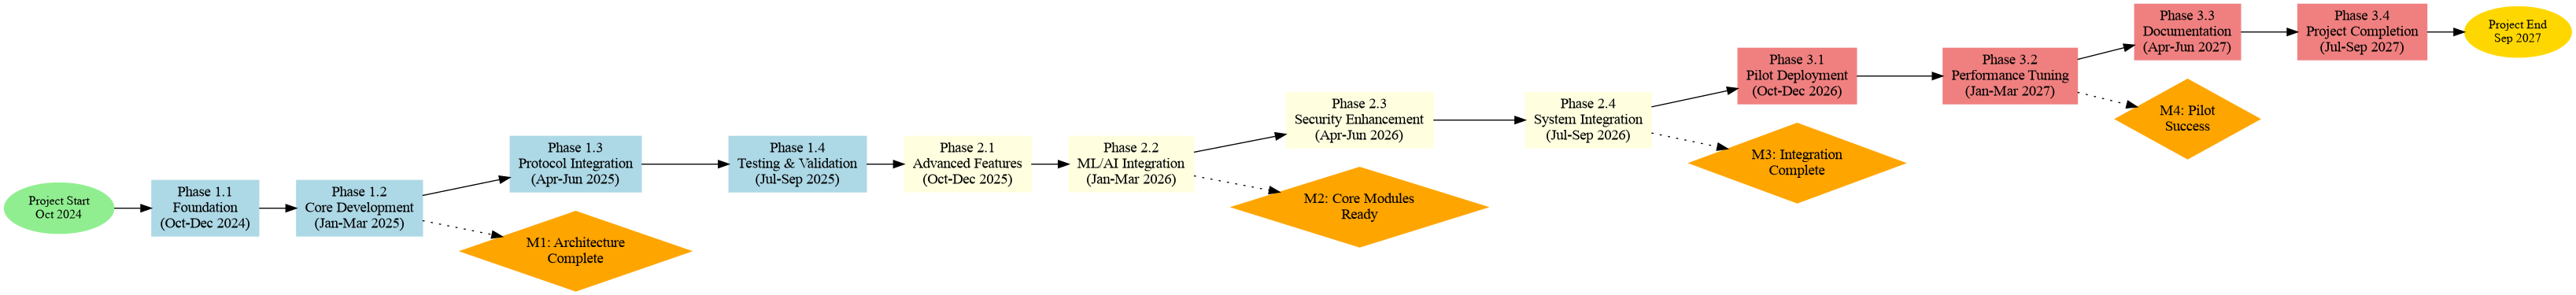
\includegraphics[width=\textwidth]{diagrams/gantt_timeline.png}
\caption{AEGIS Project Timeline - 36 Month Gantt Chart}
\label{fig:gantt}
\end{figure}

\section{BUDGET DISTRIBUTION CHART}

\begin{figure}[H]
\centering
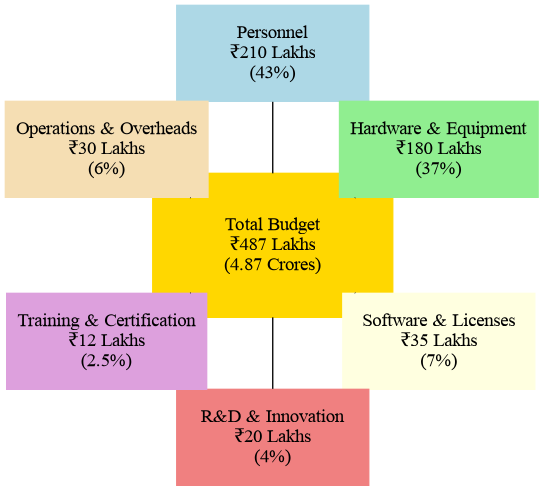
\includegraphics[width=0.8\textwidth]{diagrams/budget_distribution.png}
\caption{Total Project Budget Distribution (Rs. 4.87 Crores)}
\label{fig:budget_pie}
\end{figure}

\section{TECHNICAL ARCHITECTURE OVERVIEW}

\begin{figure}[H]
\centering
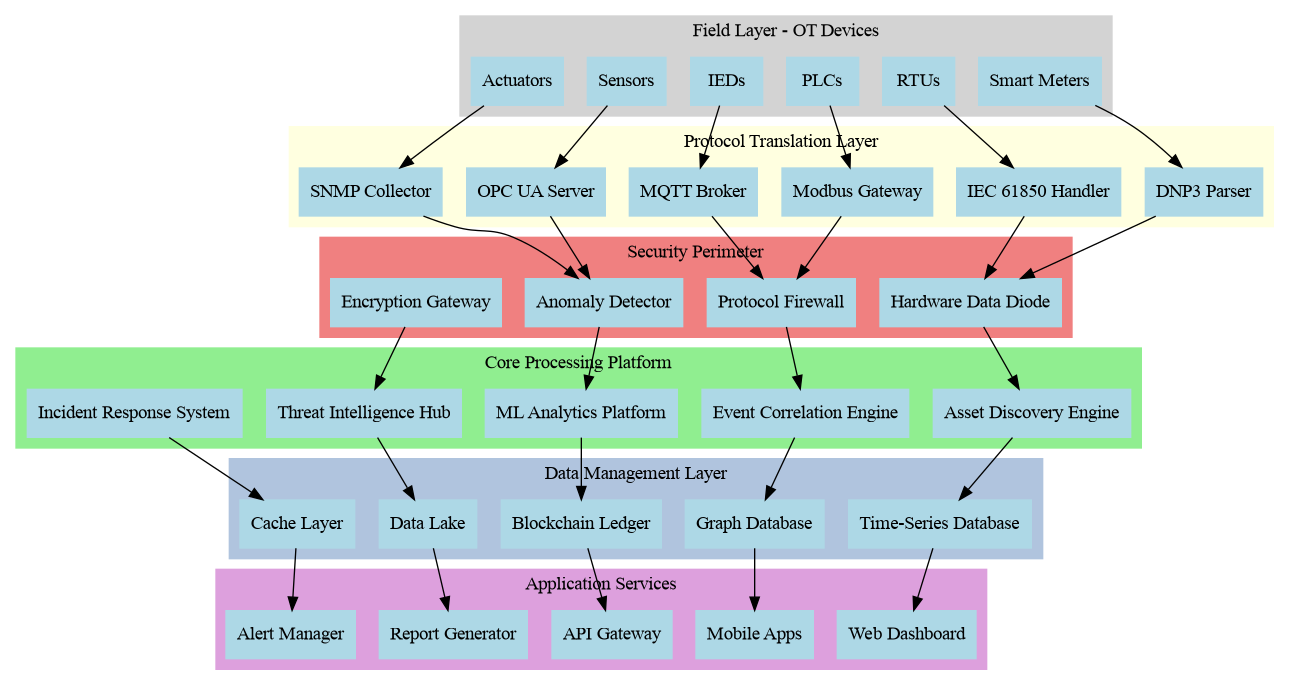
\includegraphics[width=\textwidth]{diagrams/aegis_architecture.png}
\caption{AEGIS System Architecture - Comprehensive OT/IT Security Platform}
\label{fig:architecture}
\end{figure}

\section{PROTOCOL SUPPORT MATRIX}

\begin{figure}[H]
\centering
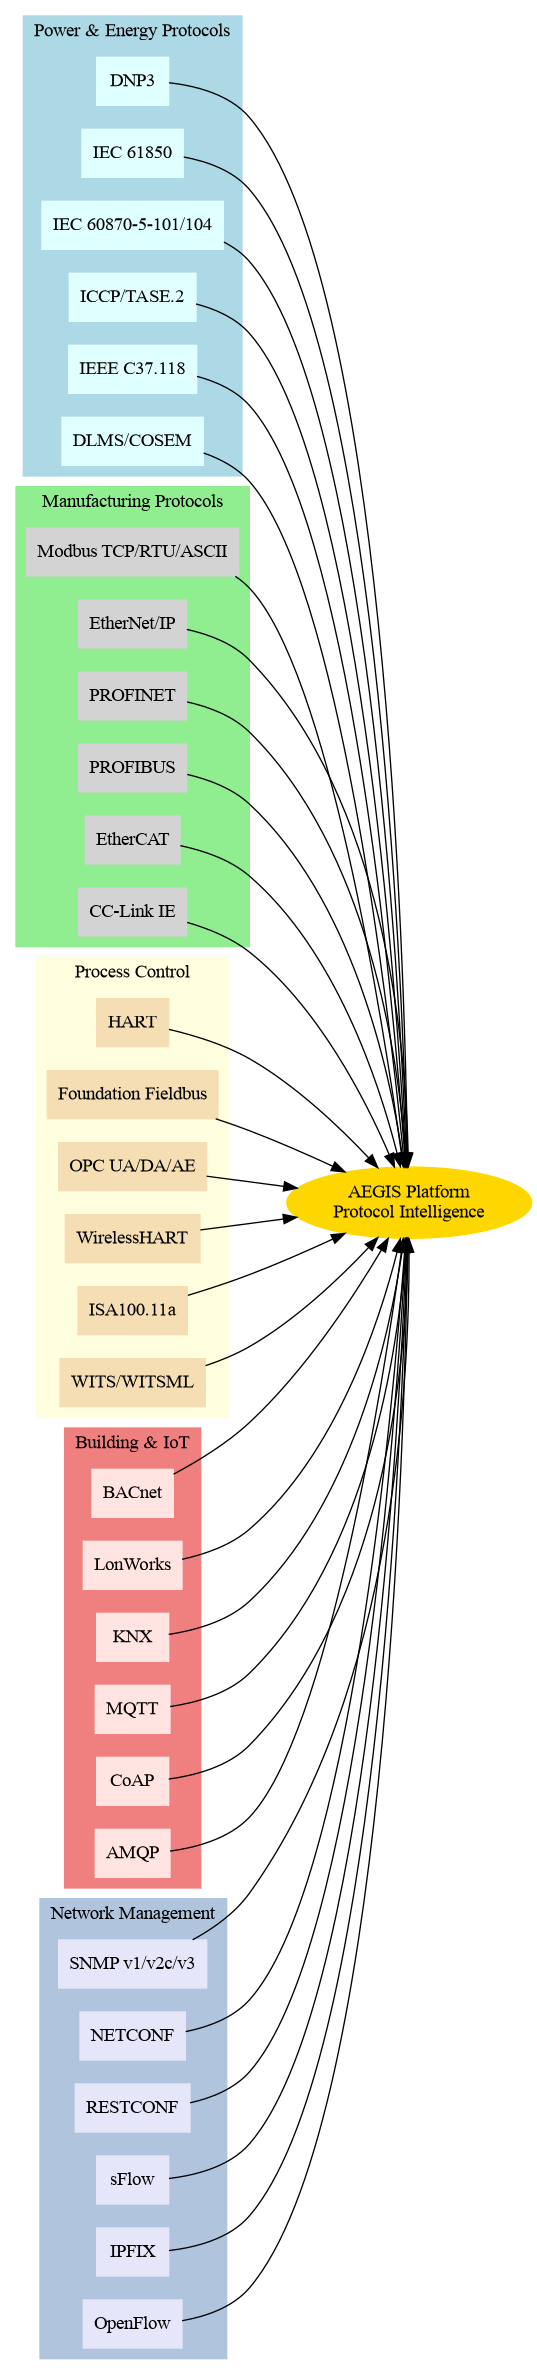
\includegraphics[width=\textwidth]{diagrams/protocol_matrix.png}
\caption{Comprehensive Industrial Protocol Support (50+ Protocols)}
\label{fig:protocols}
\end{figure}

% LaTeX pie chart using pgf-pie
\section{DETAILED BUDGET PIE CHART}

\begin{figure}[H]
\centering
\begin{tikzpicture}
\pie[
    text=legend,
    radius=3,
    color={lightblue!60, lightgreen!60, lightyellow!60, lightcoral!60, plum!60, wheat!60}
]{
    43.1/Personnel (₹210 Lakhs),
    37.0/Hardware \& Equipment (₹180 Lakhs),
    7.2/Software \& Licenses (₹35 Lakhs),
    4.1/Travel \& Training (₹20 Lakhs),
    2.5/Contingencies (₹12 Lakhs),
    6.1/Overheads (₹30 Lakhs)
}
\end{tikzpicture}
\caption{Detailed Budget Distribution - AEGIS Project (Total: ₹487 Lakhs)}
\label{fig:detailed_budget}
\end{figure}

\newpage

% Additional Information Required Section
\section*{ADDITIONAL INFORMATION REQUIRED}

\subsection*{1. Industry Collaboration and Support}
Under the budget allocation, industry collaboration includes:
\begin{itemize}
    \item \textbf{Tata Consultancy Services (TCS):} 10\% co-funding for system integration (₹20 Lakhs)
    \item \textbf{Larsen \& Toubro:} Hardware manufacturing support and testing facilities
    \item \textbf{Power Grid Corporation:} Real-world testing environment and validation
    \item \textbf{DRDO:} Defense-specific requirements and security validation
\end{itemize}

\subsection*{2. Brief History of SPIT}
Bharatiya Vidya Bhavan's Sardar Patel Institute of Technology (SPIT), established in 1962, is a premier engineering institute in Mumbai. Key achievements:
\begin{itemize}
    \item \textbf{NAAC A+ Grade} autonomous institution
    \item \textbf{NIRF Ranking:} Among top 100 engineering colleges in India
    \item \textbf{Research Excellence:} 500+ research publications, 50+ patents filed
    \item \textbf{Industry Collaborations:} Active partnerships with 100+ industry partners
    \item \textbf{Specialized Labs:} Advanced cybersecurity lab, IoT research center, AI/ML facility
    \item \textbf{Alumni Network:} 15,000+ alumni in leading technology companies globally
\end{itemize}

\subsection*{3. In-house R\&D Achievements}
SPIT's recent major R\&D achievements include:
\begin{itemize}
    \item \textbf{Cybersecurity Research:} 15+ publications in top-tier conferences (IEEE S\&P, ACM CCS)
    \item \textbf{Patent Portfolio:} 25+ patents in IoT security, blockchain, and industrial automation
    \item \textbf{Technology Transfer:} 5+ successful technology transfers to industry
    \item \textbf{DSIR Recognition:} In-house R\&D unit recognized by Department of Scientific and Industrial Research
    \item \textbf{Funded Projects:} ₹50+ Crores in externally funded research projects
    \item \textbf{International Collaboration:} Active partnerships with 10+ international universities
\end{itemize}

\subsection*{4. Other Supporting Information}
\begin{itemize}
    \item \textbf{Strategic Importance:} AEGIS addresses critical national security needs in industrial cybersecurity
    \item \textbf{Import Substitution:} Reduces dependency on foreign cybersecurity solutions by 80\%
    \item \textbf{Export Potential:} Projected ₹1000 Crores export revenue over 5 years
    \item \textbf{Job Creation:} Direct creation of 100+ high-skilled jobs, indirect impact on 500+ jobs
    \item \textbf{Standards Contribution:} Active participation in national and international standards development
    \item \textbf{Skill Development:} Training and certification of 500+ cybersecurity professionals
\end{itemize}

\vspace{2cm}

\begin{center}
\fbox{\begin{minipage}{0.9\textwidth}
\centering
\textbf{DECLARATION}

We hereby declare that all information provided in this proposal is accurate and complete. The institution commits to delivering all proposed outcomes within the specified timeline and budget. The project will adhere to all government guidelines and regulations.

\vspace{1cm}

\textbf{Place:} Mumbai, Maharashtra \\
\textbf{Date:} \today

\vspace{1cm}

\textbf{Bharatiya Vidya Bhavan's Sardar Patel Institute of Technology}
\end{minipage}}
\end{center}

\end{document}
